\documentclass[conference]{IEEEtran}
%===========================================================================================%
% PREAMBLE
%\usepackage[a4paper, portrait]{geometry}
\usepackage{fixltx2e}
		
\usepackage{amsfonts, amsmath, amssymb, amsthm}	% AMS packages
%\usepackage[foot]{amsaddr}

\usepackage{bbm, dsfont, mathrsfs}				% Fonts
\usepackage[T1]{fontenc}
\usepackage{url}

\usepackage{array, booktabs, multirow}
%\usepackage[retainorgcmds]{IEEEtrantools}		%IEEEeqnarray environment
\usepackage{mathtools}
%\usepackage{thmtools, thm-restate}	

\usepackage[usenames, svgnames, table]{xcolor}	% Placement averts 'option clash for package xcolor'

\usepackage{enumitem}
\usepackage[font=small]{caption, subcaption}
%\usepackage{footnote}
\usepackage{footmisc}						% Multiple references to the same footnote
\usepackage{fnpct}

\usepackage{afterpage, pdflscape}
\usepackage[figuresright]{rotating}
	    \setlength\rotFPtop{0pt plus 1fil}	% Required for \sidewaystable in \documentclass{amsart}
	    
\usepackage{graphicx} 
	\DeclareGraphicsRule{.tif}{png}{.png}{`convert #1 `dirname #1`/`basename #1 .tif`.png}
	\usepackage{epstopdf}
\usepackage{tikz}

\usepackage{textcomp}
\usepackage{esvect}
\setcounter{MaxMatrixCols}{20}				% Change maximum number of matrix columns
\renewcommand{\descriptionlabel}[1]{		% Change description label from "#1:" to "#1."
	\hspace\labelsep\upshape\bfseries #1.
}

%\usepackage{abstract}

\usepackage{calc}			% Performs arithmetic on the arguments of LaTeX commands
\usepackage{xargs}			% Allow definition of commands with multiple optional arguments 
\usepackage{setspace}		% Set line spacing, e.g., double line spacing for drafts

%\numberwithin{equation}{section}

%===========================================================================================%
\newcommand{\sqrts}[2][]{\,\sqrt[#1]{#2}\,}

\def\E{\mathbb{E}}
\def\el{l}
\def\given{\,|\,}
\def\I{\mathbb{I}}
\def\N{\mathbb{N}}
\def\one{\mathds{1}}
\def\P{\mathbb{P}}
\def\R{\mathbb{R}}
\def\S{\mathbb{S}}

\def\mwmwh{\delta}
\def\eff{\eta}

%===========================================================================================%
% BIBLIOGRAPHY
\usepackage[numbers]{natbib}
	\renewcommand{\bibfont}{\normalfont\small}	%Bibliography font size = small
	
%===========================================================================================%
\hyphenation{allows battery effi-ciency paper renew-able reverse vector}

%===========================================================================================%
\begin{document}

\title{Dispatchability of Wind Power with Battery\\Energy Storage in South Australia}

% Author names and affiliations (for up to three different affiliations)
\author{
\IEEEauthorblockN{Silvio Tarca, Matthew Roughan and Nigel Bean}
\IEEEauthorblockA{School of Mathematical Sciences and\\
ARC Centre of Excellence\\
for Mathematical \& Statistical Frontiers\\
The University of Adelaide\\
South Australia, 5005\\
Email: \{\url{silvio.tarca, matthew.roughan, nigel.bean}\}\\
\hspace{1.75em}\url{@adelaide.edu.au}}
%\and
%\IEEEauthorblockN{Matthew Roughan}
%\IEEEauthorblockA{School of Mathematical Sciences\\
%The University of Adelaide\\
%Adelaide, South Australia 5005}
\and
\IEEEauthorblockN{Nesimi Ertugrul}
\IEEEauthorblockA{School of Electrical \& Electronic Engineering\\
and Centre for Energy Technology\\
The University of Adelaide\\
South Australia, 5005\\
Email: \url{nesimi.ertugrul@adelaide.edu.au}}
}

% Conference papers do not typically use \thanks and this command is locked out in conference mode. If really needed, 
% such as for the acknowledgment of grants, issue a \IEEEoverridecommandlockouts after \documentclass

\maketitle

%===========================================================================================%
% ABSTRACT																					 %
%===========================================================================================%
\begin{abstract}
The Government of South Australia (SA) has pledged to increase the state's electricity generation from renewable energy sources from 41\% in fiscal year 2015 to 50\% by 2025.  At the level of intermittent renewable energy penetration in SA the challenge is to economically supply baseload power of acceptable quality.  This study measures the improvement in the dispatchability of intermittent renewable energy from an SA wind farm coupled with a utility-scale battery using model predictive control and real-world data published by the Australian Energy Market Operator.  The process of wind power dispatch with battery energy storage is represented as an incremental state-space model.  The state-space model properly accounts for battery charge/discharge efficiency, and its incremental formulation allows the controller to penalise control effort.  We find that the probability of power dispatched to the electricity grid supplying a target baseload power is moderately higher with battery energy storage than no energy storage.
\end{abstract}

% Keywords
{\small \textbf{\textit{Wind power dispatch; battery energy storage; baseload power; model predictive control; state-space model; process control law}}}

%===========================================================================================%
% INTRODUCTION																				 %
%===========================================================================================%
\section{Introduction}
The Australian Energy Market Operator (AEMO), the independent system operator of the National Electricity Market (NEM), reports that in fiscal year 2015, 41\% of 12,352 GWh of electricity generated in the state of South Australia (SA) came from intermittent renewable energy sources --- 34\% wind and 7\% solar photovoltaic (PV) \citep{SAER15}.  Through fiscal year 2015, AUD 6.6 billion had already been invested in renewable energy in SA, and the State Government set an investment target of AUD 10 billion to achieve 50\% renewable energy generation by 2025.  With the closure of SA's last two ageing coal-fired power plants in May 2016, it now seems likely that SA will reach its renewable energy generation target well in advance of 2025.  Compared with other leading international jurisdictions for renewable energy, SA ranks second behind Denmark on the share of electricity generation from wind, and second behind Germany on installed capacity of solar PV per capita \citep{SAGOV15}.  SA is a real-world laboratory for the study of intermittent renewable energy technology, economics and public policy.
%Through fiscal year 2015 the SA Government had already invested AUD 6.6 billion in renewable energy, and plans to increase its investment to AUD 10 billion to achieve its target of 50\% renewable energy generation by 2025. 

Conventional ``scheduled'' generators submit dispatch offers with the quantity of electrical power for sale by price band to the NEM, which conducts a single-price reverse auction to set dispatch levels and price.  However, due to the intermittency of wind energy, wind generators submit only price offers and AEMO determines their wind power output offered for dispatch.  Improving the dispatchability of wind power with battery energy storage could lead to a reclassification of wind farms as scheduled generators in the NEM, which would permit time shifting of wind power dispatched to the electricity grid.  This time shifting capability would enable wind generators to supply baseload power to the grid, exploit energy arbitrage, and provide ancillary services to the power system.

This paper examines the dispatchability of wind power with battery energy storage in SA using state-space model predictive control (MPC).  The contribution of this research is both theoretical and empirical.  Our theoretical contribution represents the process of wind power dispatch with battery energy storage as an incremental state-space model.  The state-space model properly accounts for battery charge/discharge efficiency, and its incremental formulation allows the MPC controller to penalise control effort.  

On an empirical level, we demonstrate the improvement in the dispatchability of intermittent renewable energy by simulating power dispatched to the grid by an SA wind farm coupled with a utility-scale battery at varying levels of confidence.  Using unconstrained intermittent generation forecasts (UIGF) produced by the Australian Wind Energy Forecasting System (AWEFS) and published by AEMO, we find that the probability of power dispatched to the grid supplying a target baseload power is moderately higher with battery energy storage than no energy storage.
%Baseload power is the minimum continuous level of operational demand, and baseload generators are power plants that can dependably supply electricity to meet that demand \citep{NS11}.

A number of recent studies use state-space MPC to demonstrate the improvement in wind power dispatch with battery energy storage.  Their common objective is to minimise the tracking error of actual power dispatched to the grid relative to set points generated using, among other data, wind power forecasts.  They implement MPC controllers that enable wind farms to: schedule power dispatched to the grid \citep{HALBB14,TBBH10}; minimise cost by prolonging battery life \citep{KS10,YCTL12}; maximise revenue by exploiting energy arbitrage \citep{KKSA13}; or supply quality power through the provision of ancillary services \citep{YCTL14}.  The state-space models developed in prior papers are not of the incremental type, and do not penalise control effort.  Nor do they properly account for battery charge/discharge efficiency, instead, either assuming 100\% efficiency or approximating power losses independent of the power stored or discharged during the dispatch interval.

%The MPC controllers developed in these papers do not penalise control effort, nor do they properly account for battery charge/discharge efficiency.  \citep{KS10} penalises the control signal, not the control increment which is generally considered as the control effort.  \citep{HALBB14} approximates power losses independent of the power stored/discharged during the dispatch interval, while the other studies assume 100\% charge/discharge efficiency.

%We begin in Section~\ref{sect:ssmpc_dispatch} by formulating the state-space MPC controller for wind power dispatch with battery energy storage.  Section~\ref{sect:sim_disp_wind_power_bess} describes real-world data for an SA wind farm published by AEMO, and specifications of battery energy storage systems that facilitate time shifting of wind power dispatch.  It proceeds to present results of computer simulations implementing a na\"ive strategy of wind power dispatch with utility-scale, lithium-ion batteries of varying sizes (i.e., power rating and energy capacity) over a target baseload power range.  We conclude by outlining the direction of future related research.

%===========================================================================================%
% STATE-SPACE MPC OF WIND POWER DISPATCH WITH BATTERY ENERGY STORAGE						 %
%===========================================================================================%
\section{State-Space MPC of Wind Power Dispatch with Battery Energy Storage}\label{sect:ssmpc_dispatch}
Our research examines the dispatchability of intermittent renewable energy by simulating power dispatched by an SA wind farm coupled with a utility-scale battery using state-space \textit{model predictive control} (MPC).  A \textit{state-space model} represents a physical process by describing its outputs as a function of state variables, which depend on control signals or process inputs.  The MPC controller determines a sequence of control signals over a given control horizon that results in a sequence of predicted process outputs over a specified prediction horizon, which tracks a sequence of set points or reference signals.  We refer to the sequence of control signals as the \textit{process control law}.  The resulting trajectory of predicted process outputs is an outcome of optimising a \textit{performance index}, or minimising a cost function, that penalises the tracking error of the predicted process outputs relative to their set-point trajectory and the control effort involved in tracking the set-point trajectory.  

MPC applies the \textit{receding horizon} principle.  At each time step, the sequence of control signals over the control horizon is determined by optimising the performance index over the prediction horizon, but only the current-time control signals are implemented.  Then, at the next time step, the MPC algorithm is rerun incorporating new non-anticipatory information with control and prediction horizons shifted one time step into the future.     

%===========================================================================================%
% Incremental State-Space Model																	 %
%===========================================================================================%
\subsection{Incremental State-Space Model}\label{sect:state_space_model}
In the incremental formulation of the state-space model, the control signals become internal state variables augmenting the observable state variables, and control increments serve as process inputs.  We begin by formulating a single-period incremental state-space model in the standard notation typically used to represent an abstract process.  Next, we define the process outputs, state variables and control signals that capture the process dynamics of wind power dispatch with battery energy storage, and formulate the representative incremental state-space model for a single period.  Finally, the single-period model is extended to accommodate multi-period prediction and control horizons.

Time in the incremental state-space model is represented as discrete time steps, or intervals, $t\in\N$.  Suppose that discrete times $t\!-\!1$ and $t$, respectively, translate to clock times $\varsigma$ and $\tau$.  Then, ``at time~$t$'' refers to clock time~$\tau$, and ``during time interval~$t$'' refers to clock time interval $(\varsigma, \tau]$.

Let ${\boldsymbol{y}(t)\in\R^{m}}$ be the process output vector at time~$t$, ${\boldsymbol{x}(t)\in\R^{s-q}}$ the observable state vector at time~$t$, and ${\boldsymbol{u}(t)\in\R^{q}}$ the control signal vector at time~$t$.  Denote by ${\boldsymbol{z}(t)\in\R^{s}}$ the augmented state vector at time~$t$, and ${\boldsymbol{\Delta{u}}(t)\in\R^{q}}$ the control increment vector at time~$t$.  Then, the single-period incremental state-space model representing an abstract process may be expressed as 
\begin{IEEEeqnarray*}{rCCCl}
	% State matrix equation
	\boldsymbol{z}(t\!+\!1) & = &
	\begin{bmatrix*}[c]
		\boldsymbol{x}(t\!+\!1)	\\
		\boldsymbol{u}(t)
	\end{bmatrix*}
	& = & A
	\begin{bmatrix*}[c]
		\boldsymbol{x}(t)		\\
		\boldsymbol{u}(t\!-\!1)
	\end{bmatrix*}
	+ B\left(\boldsymbol{u}(t) - \boldsymbol{u}(t\!-\!1)\right) \\
	& & & = & A\boldsymbol{z}(t) + B\boldsymbol{\Delta{u}}(t),	\IEEEyesnumber\label{eqn:ssm_state}\\
	% Process output matrix equation
	& & \boldsymbol{y}(t\!+\!1) & = & C\boldsymbol{z}(t\!+\!1) \\
	& & & = & CA\boldsymbol{z}(t) + CB\boldsymbol{\Delta{u}}(t),	\IEEEyesnumber\label{eqn:ssm_output}
\end{IEEEeqnarray*}
where $A\in\R^{s\times{s}}$, $B\in\R^{s\times{q}}$ and $C\in\R^{m\times{s}}$ are matrices defining the incremental state-space model.

Our incremental state-space model for wind power dispatch with battery energy storage includes two process outputs, four state variables and three control increments.  Let ${e(t) \geq 0}$ be the state of charge (SOC) of the battery at time~$t$, ${p_{b+}(t) \geq 0}$ the battery charge control signal at time~$t$, and ${p_{b-}(t) \geq 0}$ the battery discharge control signal at time~$t$.  We assume that the battery charge control signal diverts wind-generated power to the battery, while the battery discharge control signal dispatches battery power to the electricity grid.  Denote by ${\eff\in(0,1]}$ the one-way charge/discharge efficiency of the battery, and ${\mwmwh > 0}$ the conversion factor from MW to MWh for a given dispatch interval.  Then, the battery SOC is given by
\begin{IEEEeqnarray*}{rCl}
	e(t\!+\!1) & = & e(t) + {\mwmwh\eff}p_{b+}(t) -  \frac{\mwmwh}{\eff}p_{b-}(t)	.	\IEEEyesnumber\label{eqn:bess_soc}
\end{IEEEeqnarray*}
Notice that the increase in battery SOC is less than the energy diverted from the grid by the battery charge control signal over the dispatch interval by the factor of efficiency $\eff$.  Conversely, the decrease in battery SOC is greater than the energy supplied to the grid by the battery discharge control signal over the dispatch interval by the factor of efficiency $\eff$.  Also, factor $\mwmwh$ converts the battery charge/discharge control signal (MW), which applies over the dispatch interval, to energy (MWh).
%, for example, $\mwmwh = \tfrac{1}{12}$ is one-twelfth of one hour which corresponds to a 5-minute dispatch interval.

Let ${p_{d}(t) \geq 0}$ be the power dispatched from the wind farm to the grid during time interval~$t$, and ${p_{w}(t) \geq 0}$ the wind power control signal at time~$t$.  In the context of the empirical analysis presented in this paper, $p_{d}(t)$ represents \textit{baseload power}, which we broadly define as the dependable supply of electricity to meet a minimum continuous level of operational demand \citep{NS11}.  Then, power dispatched to the grid is given by
\begin{IEEEeqnarray*}{rCl}
	p_{d}(t\!+\!1) & = & p_{b-}(t) - p_{b+}(t) + p_{w}(t),\IEEEyesnumber\label{eqn:power_disp_grid}
\end{IEEEeqnarray*}
where 
\begin{equation}\label{eqn:bess_pwr_cmd}
	p_{b}(t) = p_{b-}(t) - p_{b+}(t)
\end{equation}
is the battery power control signal at time~$t$.  Hence, we follow the convention that $p_{b}(t)$ takes a positive value whenever battery power is discharged and dispatched to the grid, and takes a negative value whenever wind-generated power is diverted from the grid to charge the battery.  Decomposing the battery power control signal into charge and discharge control signals correctly accounts for battery charge/discharge efficiency, as well as accommodating different ranges for charge and discharge rates.  Note that control signals $p_{w}(t)$ and $p_{b}(t)$, and hence $p_{b+}(t)$ and $p_{b-}(t)$, resolved at time~$t$ apply during time interval~$t\!+\!1$.

Accordingly, we define the augmented state, control increment, and process output vectors at time~$t$ as
\begin{IEEEeqnarray*}{rCl}
	\boldsymbol{z}(t) & = & \begin{bmatrix*}[c] e(t) & p_{b+}(t\!-\!1) & p_{b-}(t\!-\!1) & p_{w}(t\!-\!1) \end{bmatrix*}^{T},\\
	\boldsymbol{\Delta{u}}(t) & = & \begin{bmatrix*}[c] \Delta{p_{b+}}(t) & \Delta{p_{b-}}(t) & \Delta{p_{w}}(t) \end{bmatrix*}^{T},\;\text{and}\\
	\boldsymbol{y}(t) & = & \begin{bmatrix*}[c] e(t) & p_{d}(t) \end{bmatrix*}^{T},\IEEEyesnumber\label{eqn:ssm_yzdu}
\end{IEEEeqnarray*}
respectively, where control increments $\Delta{p_{b+}}(t)$, $\Delta{p_{b-}}(t)$ and $\Delta{p_{w}}(t) \in \R$.  Notice that battery SOC is modelled as a process output and a state variable.  SOC of the battery reached at the end of the current dispatch (time) interval, a process output, is the SOC at the beginning of the next dispatch interval, a state variable.  The matrices defining the single-period incremental state-space model are then given by
\begin{IEEEeqnarray*}{rCl}
	A & = &
	\begin{bmatrix*}[c]
		1	& \mwmwh\eff	& -\mwmwh/\eff	& 0	\\
		0	& 1			& 0			& 0	\\
		0	& 0			& 1			& 0	\\
		0	& 0			& 0			& 1	\\
    	\end{bmatrix*},\\
	B & = &
	\begin{bmatrix*}[c]
		\mwmwh\eff	& -\mwmwh/\eff	& 0	\\
		1			& 0			& 0	\\
		0			& 1			& 0	\\
		0			& 0			& 1	\\
	\end{bmatrix*},\;\text{and}\\
	C & = &
	\begin{bmatrix*}[c]
		1	& 0	& 0	& 0	\\
		0	& -1	& 1	& 1	\\
	\end{bmatrix*}.\IEEEyesnumber\label{eqn:ssm_abc}
\end{IEEEeqnarray*}
We represent the process of wind power dispatch with battery energy storage by substituting \eqref{eqn:ssm_yzdu} and \eqref{eqn:ssm_abc} into incremental state-space model \eqref{eqn:ssm_state}--\eqref{eqn:ssm_output}.  This substitution leads to a single-period representation, however, our implementation of state-space MPC accommodates multi-period prediction and control horizons.  

Let $n_{y}$ be the number of time intervals or periods in the prediction horizon, and $n_{u}$ the number of time intervals in the control horizon.  Assume coincident prediction and control horizons, $n = n_{y} = n_{u}$.  Denote by $\vv{\boldsymbol{y}}_{t}\in\R^{mn}$ the process output vector over the prediction horizon starting at time~$t$, and $\vv{\boldsymbol{\Delta{u}}}_{t}\in\R^{qn}$ the control increment vector over the control horizon starting at time~$t$.  Then, the multi-period version of \eqref{eqn:ssm_output} may be expressed as 
\begin{equation}\label{eqn:ssm_output_kxldu}
	\vv{\boldsymbol{y}}_{t+1} = K\boldsymbol{z}(t) + L\vv{\boldsymbol{\Delta{u}}}_{t},
\end{equation}
where
\begin{IEEEeqnarray*}{rCl}
	\vv{\boldsymbol{y}}_{t+1} & = & \begin{bmatrix*}[c] \boldsymbol{y}(t\!+\!1) &\boldsymbol{y}(t\!+\!2) & \!\ldots\! & \boldsymbol{y}(t\!+\!n) \end{bmatrix*}^{T},\\
	\vv{\boldsymbol{\Delta{u}}}_{t} & = & \begin{bmatrix*}[c] \boldsymbol{\Delta{u}}(t) &\boldsymbol{\Delta{u}}(t\!+\!1) & \!\ldots\! & \boldsymbol{\Delta{u}}(t\!+\!n\!-\!1) \end{bmatrix*}^{T},%\IEEEyesnumber\label{eqn:ssm_ydu}
\end{IEEEeqnarray*}
and $K\in\R^{mn\times{s}}$ and $L\in\R^{mn\times{qn}}$ are matrices defining the multi-period incremental state-space model.  By recursively applying \eqref{eqn:ssm_state} and \eqref{eqn:ssm_output} over the $n$-period horizon, it follows that
\begin{IEEEeqnarray*}{rCl}
%\begin{equation}\label{eqn:ssm_kl}
	K & = &
	\begin{bmatrix*}[c]
		CA		\\
		CA^{2}	\\
		\vdots	\\
		CA^{n}
    	\end{bmatrix*},\;\text{and}\;\\
	L & = &
	\begin{bmatrix*}[c]
		CB			& 0			& 0		& \ldots			& 0		\\
		CAB			& CB			& 0		& \ldots			& 0		\\
		\vdots		& \vdots		& \multicolumn{2}{c}{\ddots}	& \vdots	\\
		CA^{n\!-\!1}B	& CA^{n\!-\!2}B	& \ldots	& CAB			& CB	
    	\end{bmatrix*}.%\IEEEyesnumber\label{eqn:ssm_kl}
%\end{equation}
\end{IEEEeqnarray*}

%===========================================================================================%
% Performance Index																			 %
%===========================================================================================%
\subsection{Performance Index and Process Constraints}\label{sect:perf_index}
The process control law is determined by optimising a performance index, which penalises tracking error and control effort.  Let $\vv{\boldsymbol{r}}_{t}\in\R^{mn}$ be the set-point, or reference signal, vector over the prediction horizon starting at time~$t$.  Then, we define the Euclidean norm ($\ell^{2}$-norm) of the predicted process outputs relative to their set points, $\lVert\vv{\boldsymbol{r}}_{t}-\vv{\boldsymbol{y}}_{t}\rVert_{2}$, as the tracking error.  Similarly, the control effort is defined as the norm of the control increments, $\lVert\vv{\boldsymbol{\Delta{u}}}_{t}\rVert_{2}$.  Optimisation of the performance index amounts to minimisation of a quadratic cost function that assigns weights to tracking error and control effort:
\begin{IEEEeqnarray*}{rCl}
    	f & = & \left\lVert\sqrts{\Omega}\left(\vv{\boldsymbol{r}}_{t+1}-\vv{\boldsymbol{y}}_{t+1}\right)\right\rVert_{2}^{2} + \lambda\left\lVert\sqrts{\Psi}\vv{\boldsymbol{\Delta{u}}}_{t}\right\rVert_{2}^{2},	\IEEEyesnumber\label{eqn:quad_cost_func}
\end{IEEEeqnarray*}
where
\begin{equation*}\label{eqn:cost_func_set_pt}
	\vv{\boldsymbol{r}}_{t+1} = \begin{bmatrix*}[c] \boldsymbol{r}(t\!+\!1) & \boldsymbol{r}(t\!+\!2) & \ldots & \boldsymbol{r}(t\!+\!n)\end{bmatrix*}^{T},
\end{equation*}
$\lambda \geq 0$ is a scalar weighting coefficient, and $\Omega\in\R^{mn\times{mn}}$ and $\Psi \in\R^{qn\times{qn}}$ are positive semidefinite diagonal weighting matrices.

MPC systematically accounts for process constraints by incorporating them into the optimisation of the performance index.  Here, constraints take the form of upper and lower bounds on observable and internal state variables:
\begin{IEEEeqnarray*}{rCCCl}
	\underline{\boldsymbol{x}} 		& \preceq	& \boldsymbol{x}(t\!+\!k)			& \preceq	& \overline{\boldsymbol{x}},	\\
	\underline{\boldsymbol{u}}		& \preceq	& \boldsymbol{u}(t\!+\!k\!-\!1)		& \preceq	& \overline{\boldsymbol{u}},\quad k = 1, \ldots, n,	\IEEEyesnumber\label{eqn:proc_constraints}
\end{IEEEeqnarray*}
%\underline{\boldsymbol{\Delta{u}}}	& \preceq	& \boldsymbol{\Delta{u}}(t\!+\!k\!-\!1)	& \preceq	& \overline{\boldsymbol{\Delta{u}}}
where the $\preceq$ operator represents the component-wise inequality between vectors.  Section~\ref{sect:sim_disp_wind_power_bess} specifies bounds on state variables including battery SOC, and battery charge and discharge rates.  Note that in our formulation of the optimisation problem we impose constraints on internal state variables $\boldsymbol{u}(t\!+\!k\!-\!1)$ in terms of control increments $\boldsymbol{\Delta{u}}(t\!+\!k\!-\!1)$ for $k = 1, \ldots, n$.
%Recall that augmented state vector ${\boldsymbol{z}(t\!+\!k) = \begin{bmatrix*}[c] \boldsymbol{x}(t\!+\!k) & \boldsymbol{u}(t\!+\!k\!-\!1) \end{bmatrix*}^{T}}$ comprises observable, $\boldsymbol{x}(t\!+\!k)$, and internal, $\boldsymbol{u}(t\!+\!k\!-\!1)$, state variables.  

Substituting for $\vv{\boldsymbol{y}}_{t+1}$ in \eqref{eqn:quad_cost_func} with \eqref{eqn:ssm_output_kxldu}, expanding the cost function, dropping the constant terms and imposing constraints \eqref{eqn:proc_constraints}, we write the quadratic program for wind power dispatch with battery energy storage in standard form:
\begin{IEEEeqnarray*}{rCl}
	\underset{\vv{\boldsymbol{\Delta{u}}}_{t}}{\operatorname{argmin}} & \quad & 
		\frac{1}{2}\vv{\boldsymbol{\Delta{u}}}_{t}^{T}\left(L^{T}\Omega{L} + \lambda\Psi\right)\vv{\boldsymbol{\Delta{u}}}_{t}\\
	& &+ \left(K\boldsymbol{z}(t) - \vv{\boldsymbol{r}}_{t+1}\right)^{T}\Omega{L}\vv{\boldsymbol{\Delta{u}}}_{t}	\\
    	\operatorname{s.t.} & & \underline{\boldsymbol{x}} \preceq \boldsymbol{x}(t\!+\!k) \preceq \overline{\boldsymbol{x}},	\\
	& & \underline{\boldsymbol{\Delta{u}}} \preceq \boldsymbol{\Delta{u}}(t\!+\!k\!-\!1) \preceq \overline{\boldsymbol{\Delta{u}}},\quad k = 1, \ldots, n.\qquad\IEEEyesnumber\label{eqn:perf_index_optm}
\end{IEEEeqnarray*}
%Note that the implementation of optimisation~\eqref{eqn:perf_index_optm} formulates constraints on state variables $\boldsymbol{z}(t\!+\!k)$ in terms of control increments $\boldsymbol{\Delta{u}}(t\!+\!k\!-\!1)$ for $k = 1, \ldots, n$.

Battery power control signal $p_{b}(t\!+\!k\!-\!1)$, given by \eqref{eqn:bess_pwr_cmd}, instructs that the battery either be charged or discharged.  So, if battery charge control signal $p_{b+}(t\!+\!k\!-\!1)>0$, then battery discharge control signal $p_{b-}(t\!+\!k\!-\!1)=0$; and if $p_{b-}(t\!+\!k\!-\!1)>0$, then $p_{b+}(t\!+\!k\!-\!1)=0$ for $k = 1, \ldots, n$.  Otherwise, \eqref{eqn:bess_soc} would overstate energy losses due to charge/discharge efficiency and erroneously calculate battery SOC, ${e(t\!+\!k)}$, while \eqref{eqn:power_disp_grid} would miscalculate power dispatched to the grid, ${p_{d}(t\!+\!k)}$.  In order to ensure that the optimal control signals computed by quadratic program~\eqref{eqn:perf_index_optm} instruct either zero charge or zero discharge of the battery, or both, we introduce an auxiliary binary variable for each time interval in the control horizon.  The binary variable indicates whether the battery charge control signal is zero or positive.  Then, \eqref{eqn:perf_index_optm} is reformulated as a mixed integer quadratic program by imposing additional constraints, which ensure linear complementarity --- battery charge and discharge control signals, ${p_{b+}(t\!+\!k\!-\!1) \geq 0}$ and ${p_{b-}(t\!+\!k\!-\!1) \geq 0}$, cannot both be different from zero at the same time.

Suppose that we wish to generate control signals that will drive the process during the next $N\in\N$ time intervals, then we require set points for $N\!+\!n\!-\!1$ discrete time steps to perform $N$ iterations of the simulation.  Recall that under the receding horizon principle, we compute a sequence of $n$ control signal vectors ${\boldsymbol{u}(t), \ldots, \boldsymbol{u}(t\!+\!n\!-\!1)}$ at each time step ${t = 0, 1, \ldots, N\!-\!1}$, but only implement the current-time control signal vector $\boldsymbol{u}(t)$.  So, set points ${\boldsymbol{r}(1), \ldots, \boldsymbol{r}(N\!+\!n\!-\!1)}$ are input to the computation of control signals ${\boldsymbol{u}(0), \boldsymbol{u}(1), \ldots, \boldsymbol{u}(N\!-\!1)}$ which, when implemented, drive process output responses ${\boldsymbol{y}(1), \ldots, \boldsymbol{y}(N)}$.

%===========================================================================================%
% SIMULATION OF WIND POWER DISPATCH WITH BATTERY ENERGY STORAGE							 %
%===========================================================================================%
\section{Simulation of Wind Power Dispatch with Battery Energy Storage}\label{sect:sim_disp_wind_power_bess}
AEMO classifies generators as ``scheduled'', ``semi-scheduled'' or ``non-scheduled'', with wind generators falling into either the semi- or non-scheduled categories.  The NEM dispatch process deducts available capacity for dispatch by non-scheduled generators from the operational demand forecast to arrive at scheduled demand.  Then, given scheduled demand, the NEM dispatch engine uses dispatch offers submitted by scheduled and semi-scheduled generators to determine generator dispatch levels and price through a single-price reverse auction.  While conventional scheduled generators submit dispatch offers with the quantity of electrical power for sale by price band, semi-scheduled wind generators submit only price offers and AEMO determines their wind power output offered for dispatch using AWEFS \citep{AEMO14b}.  Improving the dispatchability of wind power with battery energy storage could lead to a reclassification of wind farms as scheduled generators in the NEM, which would permit time shifting of wind power dispatched to the electricity grid.  It would enable wind generators to supply baseload power to the grid, exploit energy arbitrage, and provide ancillary services to the power system.

In this paper we report power system quantities on a per-unit (p.u.) basis.  The per-unit system expresses quantities in SI units as a ratio relative to base quantities, in our case, 100~MW for power and 100~MWh for energy.  We conduct an empirical analysis of the Snowtown (stage one) wind farm in the mid-north of SA.  It has a registered generation capacity of 1.0~p.u., and a capacity factor of 38\% over the simulation horizon.  We use dispatch UIGF forecasts produced by AWEFS and published by AEMO \citep{AEMO16}, which estimate the available capacity for wind power dispatch over a 5-minute horizon with a 5-minute resolution at a 5-minute frequency.  AEMO defines \textit{horizon} as how far in advance the forecast is produced, \textit{resolution} as the period over which the forecast is valid, and \textit{frequency} as how often the forecast is produced \citep{AEMO14b}.

\begin{table}[!t]
\begin{minipage}{0.5\textwidth}		% Required to handle footnotes in table
	%\centering
	\caption{Specifications of utility-scale, lithium-ion batteries used in simulations of wind power dispatch.  All quantities, except one-way battery charge/discharge efficiency $\eta$, are reported per-unit (p.u.).  Per-unit base quantities are 100~MW for power and 100~MWh for energy.}
	\label{tbl:bess_specs}
	\begin{tabular}{l r r r r}
		\toprule
		& \multicolumn{4}{c}{Lithium-ion Battery} \\
		& \multicolumn{1}{c}{(1)}	& \multicolumn{1}{c}{(2)}	& \multicolumn{1}{c}{(3)}	& \multicolumn{1}{c}{(4)}	\\
		\midrule
		Energy capacity					& 0.250	& 0.500	& 0.750	& 1.000	\\
		Power rating						& 0.125	& 0.250	& 0.375	& 0.500	\\
		Min.\ SOC,\footnote{By convention SOC of a battery is expressed as a percentage of its energy capacity, but here we report SOC per-unit.  Minimum SOC of the battery is 12.5\% of its energy capacity.} $\underline{e}$	& 0.031	& 0.062	& 0.094	& 0.125	\\
		Max.\ SOC,\footnote{Maximum SOC of the battery is 87.5\% of its energy capacity.} $\overline{e}$	& 0.219	& 0.438	& 0.656	& 0.875	\\
		Initial SOC,\footnote{Initial SOC of the battery, $e(0) = (\underline{e}+\overline{e})/2 = 50\%$ of its energy capacity.}	$e(0)$	& 0.125	& 0.250	& 0.375	& 0.500	\\
		Max.\ charge rate,\footnote{Maximum battery charge/discharge rate is 80\% of its rated power.\label{fn:max_chrg_rt}} $\overline{p}_{b+}$	& 0.100	& 0.200	& 0.300	& 0.400	\\
		Max.\ discharge rate,\footref{fn:max_chrg_rt} $\overline{p}_{b-}$	& 0.100	& 0.200	& 0.300	& 0.400	\\
		One-way charge eff., $\eff$		& 0.920	& 0.920	& 0.920	& 0.920	\\
		\bottomrule
	\end{tabular}
\end{minipage}
\end{table}

%\begin{table}[!b]
%\begin{minipage}{0.5\textwidth}		% Required to handle footnotes in table
%	%\centering
%	\caption{Specifications of utility-scale, lithium-ion batteries used in simulations of wind power dispatch.  Per-unit (p.u.) base quantities are 100~MW for power and 100~MWh for energy.}
%	\label{tbl:bess_specs}
%	\begin{tabular}{l r r r}
%		\toprule
%		& \multicolumn{3}{c}{Lithium-ion Battery} \\
%		& \multicolumn{1}{c}{(1)}	& \multicolumn{1}{c}{(2)}	& \multicolumn{1}{c}{(3)}	\\
%		\midrule
%		Energy capacity (p.u)						& 0.5000	& 0.7500	& 1.0000	\\
%		Power rating (p.u.)							& 0.2500	& 0.3750	& 0.5000	\\
%		Min.\ SOC, $\underline{e}$	(p.u.)\footnote{By convention SOC of a battery is expressed as a percentage of its energy capacity, but here we report SOC per-unit.  Minimum SOC of the battery is 12.5\% of its energy capacity.}	& 0.0625	& 0.0937	& 0.1250	\\
%		Max.\ SOC, $\overline{e}$ (p.u.)\footnote{Maximum SOC of the battery is 87.5\% of its energy capacity.}	& 0.4375	& 0.6563	& 0.8750	\\
%		Initial SOC, $e(0)$ (p.u.)\footnote{Initial SOC of the battery, $e(0) = (\underline{e}+\overline{e})/2 = 50\%$ of its energy capacity.}	& 0.2500	& 0.3750	& 0.5000	\\
%		Max.\ charge rate, $\overline{p}_{b+}$ (p.u.)\footnote{Maximum battery charge/discharge rate is 80\% of its rated power.\label{fn:max_chrg_rt}}	& 0.2000	& 0.3000	& 0.4000	\\
%		Max.\ discharge rate, $\overline{p}_{b-}$ (p.u.)\footref{fn:max_chrg_rt}	& 0.2000	& 0.3000	& 0.4000	\\
%		Charge/discharge efficiency, $\eff$		& 0.9200	& 0.9200	& 0.9200	\\
%		\bottomrule
%	\end{tabular}
%\end{minipage}
%\end{table}

\begin{figure*}[!t]
	\centering
	\caption[Dispatchability of wind power with battery energy storage]{Probability of (wind and battery) power dispatched to the grid equaling or exceeding a set point representing target baseload power.  The set point follows the daily load profile of the season, summer or winter. The MPC controller uses 5-minute dispatch data from 1 April 2015 to 31 March 2016.  Registered generation capacity of the wind farm is 1.0 p.u.  Specifications of utility-scale, lithium-ion batteries are reported in Table~\ref{tbl:bess_specs}.} 
	\label{fig:disp_wind_bess}
	\scalebox{1.0}{
		% GNUPLOT: LaTeX picture with Postscript
\begingroup
  \makeatletter
  \providecommand\color[2][]{%
    \GenericError{(gnuplot) \space\space\space\@spaces}{%
      Package color not loaded in conjunction with
      terminal option `colourtext'%
    }{See the gnuplot documentation for explanation.%
    }{Either use 'blacktext' in gnuplot or load the package
      color.sty in LaTeX.}%
    \renewcommand\color[2][]{}%
  }%
  \providecommand\includegraphics[2][]{%
    \GenericError{(gnuplot) \space\space\space\@spaces}{%
      Package graphicx or graphics not loaded%
    }{See the gnuplot documentation for explanation.%
    }{The gnuplot epslatex terminal needs graphicx.sty or graphics.sty.}%
    \renewcommand\includegraphics[2][]{}%
  }%
  \providecommand\rotatebox[2]{#2}%
  \@ifundefined{ifGPcolor}{%
    \newif\ifGPcolor
    \GPcolorfalse
  }{}%
  \@ifundefined{ifGPblacktext}{%
    \newif\ifGPblacktext
    \GPblacktexttrue
  }{}%
  % define a \g@addto@macro without @ in the name:
  \let\gplgaddtomacro\g@addto@macro
  % define empty templates for all commands taking text:
  \gdef\gplbacktext{}%
  \gdef\gplfronttext{}%
  \makeatother
  \ifGPblacktext
    % no textcolor at all
    \def\colorrgb#1{}%
    \def\colorgray#1{}%
  \else
    % gray or color?
    \ifGPcolor
      \def\colorrgb#1{\color[rgb]{#1}}%
      \def\colorgray#1{\color[gray]{#1}}%
      \expandafter\def\csname LTw\endcsname{\color{white}}%
      \expandafter\def\csname LTb\endcsname{\color{black}}%
      \expandafter\def\csname LTa\endcsname{\color{black}}%
      \expandafter\def\csname LT0\endcsname{\color[rgb]{1,0,0}}%
      \expandafter\def\csname LT1\endcsname{\color[rgb]{0,1,0}}%
      \expandafter\def\csname LT2\endcsname{\color[rgb]{0,0,1}}%
      \expandafter\def\csname LT3\endcsname{\color[rgb]{1,0,1}}%
      \expandafter\def\csname LT4\endcsname{\color[rgb]{0,1,1}}%
      \expandafter\def\csname LT5\endcsname{\color[rgb]{1,1,0}}%
      \expandafter\def\csname LT6\endcsname{\color[rgb]{0,0,0}}%
      \expandafter\def\csname LT7\endcsname{\color[rgb]{1,0.3,0}}%
      \expandafter\def\csname LT8\endcsname{\color[rgb]{0.5,0.5,0.5}}%
    \else
      % gray
      \def\colorrgb#1{\color{black}}%
      \def\colorgray#1{\color[gray]{#1}}%
      \expandafter\def\csname LTw\endcsname{\color{white}}%
      \expandafter\def\csname LTb\endcsname{\color{black}}%
      \expandafter\def\csname LTa\endcsname{\color{black}}%
      \expandafter\def\csname LT0\endcsname{\color{black}}%
      \expandafter\def\csname LT1\endcsname{\color{black}}%
      \expandafter\def\csname LT2\endcsname{\color{black}}%
      \expandafter\def\csname LT3\endcsname{\color{black}}%
      \expandafter\def\csname LT4\endcsname{\color{black}}%
      \expandafter\def\csname LT5\endcsname{\color{black}}%
      \expandafter\def\csname LT6\endcsname{\color{black}}%
      \expandafter\def\csname LT7\endcsname{\color{black}}%
      \expandafter\def\csname LT8\endcsname{\color{black}}%
    \fi
  \fi
    \setlength{\unitlength}{0.0500bp}%
    \ifx\gptboxheight\undefined%
      \newlength{\gptboxheight}%
      \newlength{\gptboxwidth}%
      \newsavebox{\gptboxtext}%
    \fi%
    \setlength{\fboxrule}{0.5pt}%
    \setlength{\fboxsep}{1pt}%
\begin{picture}(8162.00,5442.00)%
    \gplgaddtomacro\gplbacktext{%
      \csname LTb\endcsname%
      \put(814,704){\makebox(0,0)[r]{\strut{}0}}%
      \put(814,1151){\makebox(0,0)[r]{\strut{}10}}%
      \put(814,1599){\makebox(0,0)[r]{\strut{}20}}%
      \put(814,2046){\makebox(0,0)[r]{\strut{}30}}%
      \put(814,2493){\makebox(0,0)[r]{\strut{}40}}%
      \put(814,2941){\makebox(0,0)[r]{\strut{}50}}%
      \put(814,3388){\makebox(0,0)[r]{\strut{}60}}%
      \put(814,3835){\makebox(0,0)[r]{\strut{}70}}%
      \put(814,4282){\makebox(0,0)[r]{\strut{}80}}%
      \put(814,4730){\makebox(0,0)[r]{\strut{}90}}%
      \put(814,5177){\makebox(0,0)[r]{\strut{}100}}%
      \put(946,484){\makebox(0,0){\strut{}0.00}}%
      \put(1855,484){\makebox(0,0){\strut{}0.10}}%
      \put(2764,484){\makebox(0,0){\strut{}0.20}}%
      \put(3674,484){\makebox(0,0){\strut{}0.30}}%
      \put(4583,484){\makebox(0,0){\strut{}0.40}}%
      \put(5492,484){\makebox(0,0){\strut{}0.50}}%
      \put(6401,484){\makebox(0,0){\strut{}0.60}}%
      \put(7310,484){\makebox(0,0){\strut{}0.70}}%
    }%
    \gplgaddtomacro\gplfronttext{%
      \csname LTb\endcsname%
      \put(176,2940){\rotatebox{-270}{\makebox(0,0){\strut{}$\P\left(\text{power dispatched} \geq \text{set point}\right)$, \%}}}%
      \put(4355,154){\makebox(0,0){\strut{}Average of set points for power dispatched to the grid, p.u.}}%
      \csname LTb\endcsname%
      \put(1894,1936){\makebox(0,0)[l]{\strut{}No energy storage}}%
      \csname LTb\endcsname%
      \put(1894,1716){\makebox(0,0)[l]{\strut{}Battery (1), energy capacity = 0.25 p.u.}}%
      \csname LTb\endcsname%
      \put(1894,1496){\makebox(0,0)[l]{\strut{}Battery (2), 0.50 p.u.}}%
      \csname LTb\endcsname%
      \put(1894,1276){\makebox(0,0)[l]{\strut{}Battery (3), 0.75 p.u.}}%
      \csname LTb\endcsname%
      \put(1894,1056){\makebox(0,0)[l]{\strut{}Battery (4), 1.00 p.u.}}%
      \csname LTb\endcsname%
      \put(4846,4506){\makebox(0,0)[l]{\strut{}Capacity factor = 0.38}}%
      \put(4846,4730){\makebox(0,0)[l]{\strut{}Registered capacity = 1.0 p.u.}}%
    }%
    \gplbacktext
    \put(0,0){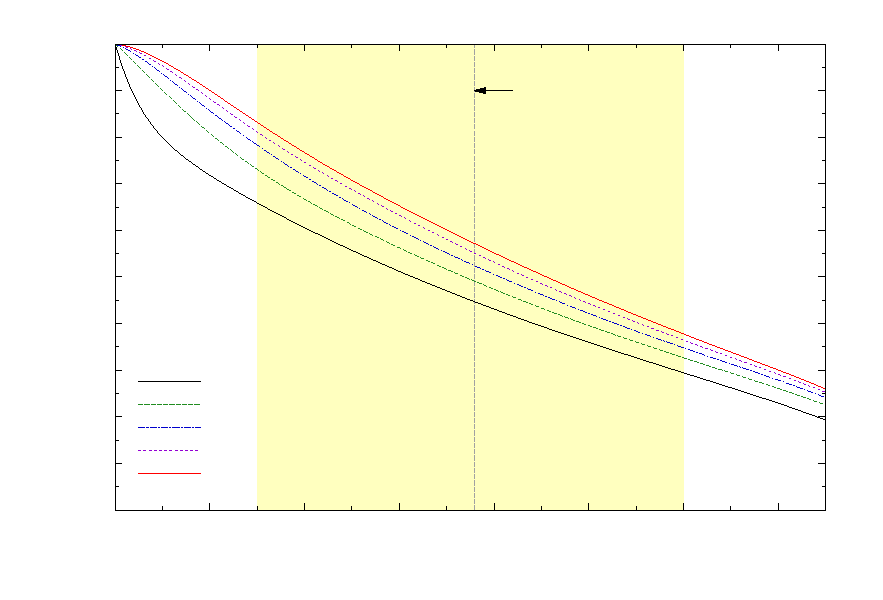
\includegraphics{plot_disp_wind_bess}}%
    \gplfronttext
  \end{picture}%
\endgroup

	}
\end{figure*}

While the Snowtown wind farm has not installed an energy storage system, we suppose that energy storage is provided by a lithium-ion battery.  Computations are repeated for four utility-scale batteries of varying energy capacity and power rating.  Their specifications are reported in Table~\ref{tbl:bess_specs}.  These specifications are not taken from existing battery installations, but they are in the bounds of current technology.  Subject to a 75\% discharge cycle, each utility-scale battery coupled to the SA wind farm can supply electricity at its rated power for one and a half hours.

Our empirical analysis implements a na\"ive dispatch strategy over single-period prediction and control horizons, $n=1$.  Subject to constraints on battery SOC and charge/discharge rates, the strategy charges the battery with surplus wind power whenever the available capacity for dispatch exceeds the set point, and discharges the battery to supplement wind power whenever the available capacity for dispatch is less than the set point.  Simulations compute control signals for $N$~=~105,408 5-minute dispatch intervals from 1 April 2015 to 31 March 2016.  It follows that the conversion factor from MW to MWh for a 5-minute dispatch interval is $\mwmwh = \tfrac{1}{12}$.  

In the state-space model, process outputs $e(t\!+\!1)$ and $p_{d}(t\!+\!1)$ depend on control signals $p_{b+}(t)$, $p_{b-}(t)$ and $p_{w}(t)$.  The wind power control signal, $p_{w}(t)$, is set to the UIGF forecast produced by AWEFS over horizon~$t$ with resolution~$t\!+\!1$.  For each dispatch interval, optimisation of the performance index determines the battery charge control signal, $p_{b+}(t)$, and battery discharge control signal, $p_{b-}(t)$, by minimising the tracking error of power dispatched to the grid, $p_{d}(t\!+\!1)$, relative to a set point that follows the daily load profile of the season, summer or winter.  In these simulations, performance index~\eqref{eqn:quad_cost_func} does not penalise the tracking error of SOC of the battery, $e(t\!+\!1)$, relative to its set point, nor does it penalise control effort, $\boldsymbol{\Delta{u}}(t)$.
%That is, the diagonal elements of $\Omega$ corresponding to battery SOC are set to zero, and $\lambda = 0$.  

Figure~\ref{fig:disp_wind_bess} illustrates the improvement in wind power dispatch with battery energy storage relative to no energy storage by plotting the probability of power dispatched to the grid equaling or exceeding a set point representing target baseload power.  Note that the ordinates of the curves in Figure~\ref{fig:disp_wind_bess} are plotted against the average of the set points (abscissas) over the simulation horizon, which are calibrated to the daily load profile of the season.  Consider a target baseload range from 0.15~p.u.\ to 0.60~p.u.\ centred on the capacity factor of the Snowtown wind farm (0.38).  Then, depending on the specifications of the battery, the number of 5-minute dispatch intervals over one full year where power dispatched to the grid equals or exceeds the set point is 10--28\% higher with a utility-scale battery than no energy storage.

%===========================================================================================%
% DISCUSSION																				 %
%===========================================================================================%
%\section{Discussion}\label{sect:discussion}
The empirical observations discussed here are made in the context of the na\"ive, single-period dispatch strategy described above.  Some observations may not, indeed, are unlikely to apply in general.  In particular, under the na\"ive strategy, the probability of power dispatched to the grid supplying a target baseload power is not very sensitive to the shape of the load profile or battery charge/discharge efficiency due to the positive autocorrelation of wind power over dispatch intervals.  In relation to the latter parameter, lower capital investment in less efficient energy storage technologies would be weighed against revenue foregone from energy losses.  We stress that these observations may not hold for other measures of dispatchability, or more sophisticated, multi-period dispatch strategies.

%In particular, under the na\"ive strategy, the probability of power dispatched to the grid supplying a target baseload power is not very sensitive to some parameters, such as battery charge/discharge efficiency or shape of the load profile, due to the positive autocorrelation of wind power over dispatch intervals.  However, this may not be the case for other measures of dispatchability, or more sophisticated dispatch strategies.

Clearly, the magnitude of the improvement in the dispatchability of wind power with battery energy storage depends on the size of the battery (energy capacity and power rating).  But, even on today's utility scale, battery power can only substitute for a fraction of the power generated by a commercial wind farm for a limited time.  For example, a utility-scale battery with energy capacity of 0.50 p.u.\ and power rating of 0.25 p.u.\ subjected to a 75\% discharge cycle can only supply electricity at its rated power for one and a half hours.  Observe, too, that the improvement in wind power dispatch with battery energy storage diminishes with increasing battery size.

We remark that this paper does not attempt to make the economic case for installing utility-scale batteries to facilitate time shifting of wind power dispatched to the grid.  But, as the cost of battery energy storage continues to tumble, utility-scale batteries may become commercially viable in the near- to medium-term.

\begin{figure}[!t]
	\centering
	\caption[Normalised load profile for typical summer day]{Normalised load profile for typical summer day in South Australia during fiscal year 2015 --- the average load during a typical summer day is equal to 1.0.	\protect\\
		{\footnotesize Source: Australian Energy Market Operator.}} 
	\label{fig:load_prof_norm_summer}
	\scalebox{0.61}{
		% GNUPLOT: LaTeX picture with Postscript
\begingroup
  \makeatletter
  \providecommand\color[2][]{%
    \GenericError{(gnuplot) \space\space\space\@spaces}{%
      Package color not loaded in conjunction with
      terminal option `colourtext'%
    }{See the gnuplot documentation for explanation.%
    }{Either use 'blacktext' in gnuplot or load the package
      color.sty in LaTeX.}%
    \renewcommand\color[2][]{}%
  }%
  \providecommand\includegraphics[2][]{%
    \GenericError{(gnuplot) \space\space\space\@spaces}{%
      Package graphicx or graphics not loaded%
    }{See the gnuplot documentation for explanation.%
    }{The gnuplot epslatex terminal needs graphicx.sty or graphics.sty.}%
    \renewcommand\includegraphics[2][]{}%
  }%
  \providecommand\rotatebox[2]{#2}%
  \@ifundefined{ifGPcolor}{%
    \newif\ifGPcolor
    \GPcolorfalse
  }{}%
  \@ifundefined{ifGPblacktext}{%
    \newif\ifGPblacktext
    \GPblacktexttrue
  }{}%
  % define a \g@addto@macro without @ in the name:
  \let\gplgaddtomacro\g@addto@macro
  % define empty templates for all commands taking text:
  \gdef\gplbacktext{}%
  \gdef\gplfronttext{}%
  \makeatother
  \ifGPblacktext
    % no textcolor at all
    \def\colorrgb#1{}%
    \def\colorgray#1{}%
  \else
    % gray or color?
    \ifGPcolor
      \def\colorrgb#1{\color[rgb]{#1}}%
      \def\colorgray#1{\color[gray]{#1}}%
      \expandafter\def\csname LTw\endcsname{\color{white}}%
      \expandafter\def\csname LTb\endcsname{\color{black}}%
      \expandafter\def\csname LTa\endcsname{\color{black}}%
      \expandafter\def\csname LT0\endcsname{\color[rgb]{1,0,0}}%
      \expandafter\def\csname LT1\endcsname{\color[rgb]{0,1,0}}%
      \expandafter\def\csname LT2\endcsname{\color[rgb]{0,0,1}}%
      \expandafter\def\csname LT3\endcsname{\color[rgb]{1,0,1}}%
      \expandafter\def\csname LT4\endcsname{\color[rgb]{0,1,1}}%
      \expandafter\def\csname LT5\endcsname{\color[rgb]{1,1,0}}%
      \expandafter\def\csname LT6\endcsname{\color[rgb]{0,0,0}}%
      \expandafter\def\csname LT7\endcsname{\color[rgb]{1,0.3,0}}%
      \expandafter\def\csname LT8\endcsname{\color[rgb]{0.5,0.5,0.5}}%
    \else
      % gray
      \def\colorrgb#1{\color{black}}%
      \def\colorgray#1{\color[gray]{#1}}%
      \expandafter\def\csname LTw\endcsname{\color{white}}%
      \expandafter\def\csname LTb\endcsname{\color{black}}%
      \expandafter\def\csname LTa\endcsname{\color{black}}%
      \expandafter\def\csname LT0\endcsname{\color{black}}%
      \expandafter\def\csname LT1\endcsname{\color{black}}%
      \expandafter\def\csname LT2\endcsname{\color{black}}%
      \expandafter\def\csname LT3\endcsname{\color{black}}%
      \expandafter\def\csname LT4\endcsname{\color{black}}%
      \expandafter\def\csname LT5\endcsname{\color{black}}%
      \expandafter\def\csname LT6\endcsname{\color{black}}%
      \expandafter\def\csname LT7\endcsname{\color{black}}%
      \expandafter\def\csname LT8\endcsname{\color{black}}%
    \fi
  \fi
    \setlength{\unitlength}{0.0500bp}%
    \ifx\gptboxheight\undefined%
      \newlength{\gptboxheight}%
      \newlength{\gptboxwidth}%
      \newsavebox{\gptboxtext}%
    \fi%
    \setlength{\fboxrule}{0.5pt}%
    \setlength{\fboxsep}{1pt}%
\begin{picture}(8162.00,5442.00)%
    \gplgaddtomacro\gplbacktext{%
      \csname LTb\endcsname%
      \put(594,503){\makebox(0,0)[r]{\strut{}0.0}}%
      \put(594,1114){\makebox(0,0)[r]{\strut{}0.2}}%
      \put(594,1725){\makebox(0,0)[r]{\strut{}0.4}}%
      \put(594,2336){\makebox(0,0)[r]{\strut{}0.6}}%
      \put(594,2948){\makebox(0,0)[r]{\strut{}0.8}}%
      \put(594,3559){\makebox(0,0)[r]{\strut{}1.0}}%
      \put(594,4170){\makebox(0,0)[r]{\strut{}1.2}}%
      \put(594,4781){\makebox(0,0)[r]{\strut{}1.4}}%
      \put(789,220){\makebox(0,0){\strut{}00:00}}%
      \put(1383,220){\makebox(0,0){\strut{}02:00}}%
      \put(1976,220){\makebox(0,0){\strut{}04:00}}%
      \put(2570,220){\makebox(0,0){\strut{}06:00}}%
      \put(3164,220){\makebox(0,0){\strut{}08:00}}%
      \put(3758,220){\makebox(0,0){\strut{}10:00}}%
      \put(4351,220){\makebox(0,0){\strut{}12:00}}%
      \put(4945,220){\makebox(0,0){\strut{}14:00}}%
      \put(5539,220){\makebox(0,0){\strut{}16:00}}%
      \put(6132,220){\makebox(0,0){\strut{}18:00}}%
      \put(6726,220){\makebox(0,0){\strut{}20:00}}%
      \put(7320,220){\makebox(0,0){\strut{}22:00}}%
    }%
    \gplgaddtomacro\gplfronttext{%
      \csname LTb\endcsname%
      \put(4277,5111){\makebox(0,0){\strut{}Normalised summer load profile}}%
    }%
    \gplbacktext
    \put(0,0){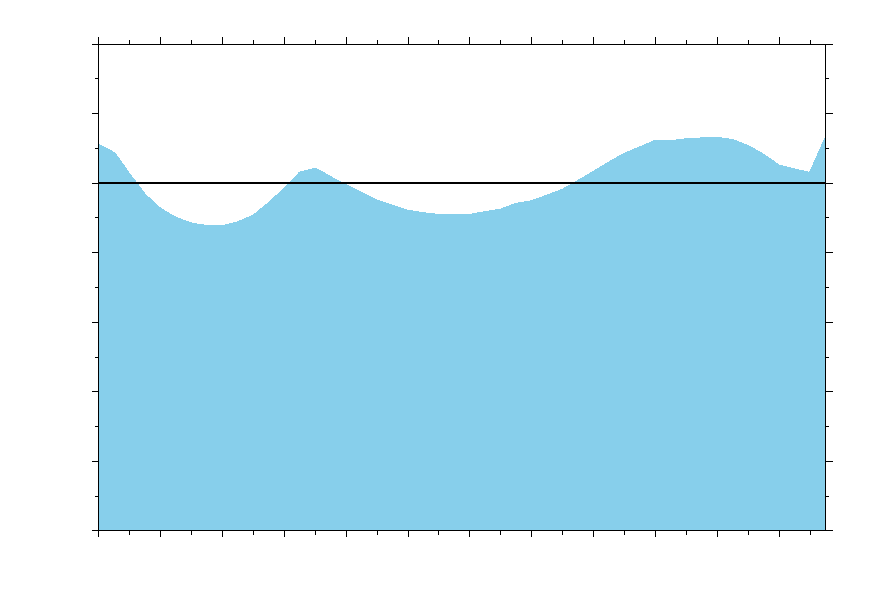
\includegraphics{plot_load_prof_summer_norm}}%
    \gplfronttext
  \end{picture}%
\endgroup

	}
\end{figure}

%As noted previously, the simulations reported in this paper implement a na\"ive strategy with single-period prediction and control horizons.  A more sophisticated strategy would store excess renewable energy during periods of low demand, and discharge the stored energy for dispatch to the grid during periods of high demand, say, between 4:00~pm and 9:00~pm.  This latter strategy requires UIGF forecasts determined by AWEFS over a prediction horizon covering the pre-dispatch period\footnote{
%The trading day comprises 48 half-hourly periods commencing from the 04:00:01--04:30:00 trading interval, designated by the end time of the period, that is, the 4:30 am trading interval.  The 40-hour pre-dispatch period commences with the 12:30 pm trading interval on the day before the actual trading day to which the dispatch offers apply \citep[AEMO,][]{AEMO10}.
%} to generate a sequence of $n_{y}$ reference signals for power dispatched to the grid that applies over an $n_{u}$-period (i.e., multi-period) control horizon.  Presumably prices would be higher during peak demand periods, so time shifting of wind power dispatched to the grid would fetch higher revenue for the wind generator owner/operator.  Moveover, if AEMO's pre-dispatch and dispatch process \citep[AEMO,][]{AEMO10} permitted wind generators to submit their dispatch offers with the quantity of electrical power for sale by price band, as conventional generators do, then wind generators could schedule power dispatched to the grid taking into account UIGF forecasts and SOC of the battery coupled to the wind farm.  The time series of power scheduled for dispatch would then become the reference signal of the MPC controller.

%===========================================================================================%
% CONCLUSION																				 %
%===========================================================================================%
\section{Conclusion}\label{sect:conclusion}
In this paper we model the process of wind power dispatch with battery energy storage using state-space MPC.  The state-space model properly accounts for battery charge/discharge efficiency, and its incremental formulation allows the controller to penalise control effort.  In simulations of power dispatched to the electricity grid by an SA wind farm coupled with a battery energy storage system, the MPC controller implements a na\"ive, single-period strategy.  Simulations are run for utility-scale batteries of varying size (energy capacity and power rating) which, subject to constraints on SOC, can supply electricity at their rated power for one and a half hours.  Over one full year using 5-minute dispatch UIGF forecasts, we find that the probability of power dispatched to the grid equaling or exceeding a set point representing target baseload power increases by 10--28\%, depending on battery size.

An obvious extension to the empirical study of this paper, which we leave for future research, would incorporate multi-period prediction and control horizons, facilitating the implementation of more sophisticated dispatch strategies.  For example, one that stores surplus intermittent renewable energy during periods of low demand, and discharges the stored energy for dispatch to the grid during periods of high demand when, presumably, prices would be higher.  Wind generators could then schedule power dispatched to the grid by taking into account multi-period UIGF forecasts and SOC of the battery, and accordingly submit their dispatch offers with the quantity of electrical power for sale by price band during pre-dispatch and dispatch.  It would allow them to exploit energy arbitrage.  Moreover, battery energy storage would enable wind generators to participate in ancillary services markets by providing the frequency (active power) and voltage (reactive power) regulation that ensures the supply of quality power \citep{ABLFJD12}.  As well as extending the dispatch strategy to incorporate multi-period prediction and control horizons, future research could examine the effect of the selection of utility-scale batteries on the performance of dispatch strategies.

%===========================================================================================%
% ACKNOWLEDGEMENTS																		 %
%===========================================================================================%
\section*{Acknowledgments}
Funding for this research is provided by the Australian Research Council through Grant \textit{CE140100049}, and the Australian Renewable Energy Agency through Grant \textit{A00720}.

%===========================================================================================%
% REFERENCES																				 %
%===========================================================================================%
\bibliographystyle{chicago}
\bibliography{sagridnat}

\end{document}


